\section{Natural language processing}
\label{sec:nlp}

% inroduction and why interesting
Natural language processing (NLP) aims to read text or listen to speech and extract meaningful information from it.
One deviation from this definition is natural language generation, where text is generated.
The difficulty in NLP is that humans for every word activate ``a cascade of semantically related concepts, relevant episodes, and sensory experiences''~\citep{cambria2014jumping}.
These activations may also differ per context.
For example, the activations for ``I want more money.'' depend on whether the sentence is uttered by a child or employee.
The field is often associated with artificial intelligence (AI).
AI is defined as ``a system's ability to correctly interpret external data, to learn from such data, and to use those learnings to achieve specific goals and tasks through flexible adaptation'' by~\citep{kaplan2019siri}.
By this definition modern NLP approaches are AI, specifically artificial narrow intelligence~\citep{kaplan2019siri}.

% tasks
The field is divided in tasks.
Some well-known tasks are:
\begin{itemize}
    \item Translating texts or \textbf{machine translation}.
    \item \textbf{Question answering} which is NLP on question sentences only.
    \item Classifying words or parts of sentences is done by \textbf{part-of-speech tagging} (for example, nouns and verbs) and \textbf{named-entity recognition} (for example, dates and locations).
    \item \textbf{Optical character recognition} attempts to recognize characters in images and can use NLP knowledge to improve accuracy.
    \item Finding co-references like ``The \underline{house} is white, and \underline{it} is located on a hill.'' is done using \textbf{coreference resolution}.
    \item NLP is not limited to text, because it includes \textbf{speech recognition} which transforms speech to text.
    \item \textbf{Entailment classification} contains examples such as ``People formed a line at the end of Pennsylvania Avenue.'' which is contained in (logically implied by) ``At the other end of Pennsylvania Avenue, people began to line up for a White House tour.''~\cite{williams2018}
    \item Determining whether two sentences have the same meaning is called \textbf{semantic text similarity}.
    \item \textbf{Sentence classification} is the broad tasks of classifying a sentence (for example, the sentiment or intention of user)
\end{itemize}
Intent classification, machine translation and named-entity recognition are introduced in Section~\ref{subsec:mt} and~\ref{subsec:nlu}.

\subsection{Language model}
\label{subsec:language_model}
To be able to explain more complex language representations using neural network architectures we first take a look at a simple statistical language model.
Language models try to capture the grammar of a language.
Capturing grammar can be done by using probabilities for sentences or probabilities of upcoming words given a part of a sentence.
It is based on the assumption that grammatically correct sentences occur more often than incorrect sentences.
The following three tasks and examples demonstrate the usefulness of probabilities.
\begin{center}
    \begin{tabular}{l l}
        Spell correction & $P(\text{my car broke}) > P(\text{my car boke})$\\
        Machine translation & $P(\text{the green house}) > P(\text{the house green})$\\
        Speech recognition & $P(\text{the red car}) > P(\text{she read ar})$
    \end{tabular}\\
\end{center}
In the first example it is much more likely that the third word should be `broke' than `boke'.
This is used by automatic spell checkers to correct mistakes.
In machine translation knowledge about the expected order of words is used to improve translation accuracy.
The speech recognition example shows that ambiguity introduced by phonetic similarity can be solved by choosing the most likely phrase.

A simple approach is to use counters to calculate the sentence probabilities.
This makes use of the chain rule or `general product rule'.
Let $W$ denote a sentence, or equivalently, sequence of words.
For the probability of the sentence we have $P(W) = P(w_1, w_2, \ldots, w_n)$.
The probability of the upcoming word $w_i$ is $P(w_i) = P(w_i \: | \: w_1, w_2, \ldots, w_{i-1})$.
Using the chain rule we can, for three variables, state that $P(w_3, w_2, w_1) = P(w_3 \: | \: w_2, w_1) \cdot P(w_2 \: | \: w_1) \cdot P(w_1)$.
This pattern scales to any number of variables.
To get the probability for the sentence `the car broke` we rewrite it as follows.
\[ P(\text{the car broke}) = P(\text{the}) \cdot P(\text{car} \: | \: \text{the}) \cdot P(\text{broke} \: | \: \text{the car}) \]
Each term can be rewritten to a combination of counters, for example: $P(\text{broke} \: | \: \text{the car}) = \textsc{count}(\text{the car}) \: / \: \textsc{count}(\text{broke})$.
This does not scale well.
The counters for each word and each pair of words are feasible.
However, when doing this for long sentences the number of counters to keep track of becomes too large.

To reduce the number of counters an approximation defined by Markov is used.
Markov states that only looking at a fixed number of previous words gives an approximation.
Considering only one previous word for our example we get the following.
\[ P(\text{broke} \: | \: \text{the car}) \approx P(\text{broke} \: | \: \text{car}) \]
This is called the bigram model.
When using this to generate sentences it becomes clear that bigrams do not have enough information.
Take the generated sentence ``I cannot betray a trust of them.''~\citep{langkilde1998practical}.
Each pair of sequential words is correct, while the sentence as a whole is not.
This simplification of looking at a fixed number of previous words is called n-grams.
Although n-grams offer good performance for certain cases they are in practise not able to capture long-distance dependencies in texts.

\subsection{Machine translation}
\label{subsec:mt}
% introduction
Machine translation became known to the public by introduction of Google Translate in 2006.
The system was based on a statistical language model (as explained in Section~\ref{subsec:language_model}) and not on a rule-based model.
Rule-based means formulating linguistic rules which is ``a difficult job and requires a linguistically trained staff''~\citep{sumita1991experiments}.
In an attempt to visualise the progress made in the field we consider one example translation through time as recorded by~\citet{manning2017lectures}.
This `one sentence benchmark' contains one Chinese to English example which is compared with Google Translate output.
The correct translation for the example is:\\

In 1519, six hundred Spaniards landed in Mexico to conquer the Aztec Empire with a population of a few million.
They lost two thirds of their soldiers in the first clash.\\

Google Translate returned the following translations.

\begin{description}
    \item[2009] 1519 600 Spaniards landed in Mexico, millions of people to conquer the Aztec empire, the first two-thirds of soldiers against their loss.
    \item[2011] 1519 600 Spaniards landed in Mexico, millions of people to conquer the Aztec empire, the initial loss of soldiers, two thirds of their encounters.
    \item[2013] 1519 600 Spaniards landed in Mexico to conquer the Aztec empire, hundreds of millions of people, the initial confrontation loss of soldiers two-thirds.
    \item[2014-2016] 1519 600 Spaniards landed in Mexico, millions of people to conquer the Aztec empire, the first two-thirds of the loss of soldiers they clash.
    \item[2017] In 1519, 600 Spaniards landed in Mexico, to conquer the millions of people of the Aztec empire, the first confrontation they killed two-thirds.
\end{description}

% alignment
One important concept in machine translation is alignment.
Alignment refers to the fact that words in different languages tend to be located at similar parts in the sentence.
Consider the sentences

\begin{center}
    ``\underline{well i think if we} can make it \underline{at eight on both days}''
\end{center}
and
\begin{center}
    ``\underline{ja ich denke wenn wir} das hinkriegen \underline{an beiden tagen acht uhr}''.
\end{center}
\vspace*{1mm}
The first five words of the sentences are perfectly aligned.
The last five words of the sentences are not.
Alignment is visualised in Figure~\ref{fig:alignment}.
Non-perfect alignment can also be observed from the fact that the number of words in English sentence is higher.

\begin{figure}[htbp]
    \begin{center}
        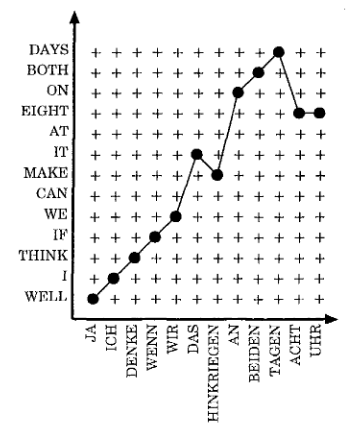
\includegraphics[scale=0.4]{figures/alignment.png}
        \vspace*{-2mm}
    \end{center}
    \caption{Word alignment for a German-English sentence pair~\cite[Figure 1]{vogel1996hmm}.}
    \label{fig:alignment}
\end{figure}

\subsection{Natural language understanding}
\label{subsec:nlu}
Conversational agent or dialogue systems aim to communicate with humans using natural language.
Consensus is not clear on whether a chatbot is synonymous to conversational agent.
Some argue it is~\citep{io2017chatbots}, and some argue that conversational agents are more sophisticated that bots which can chat.
This thesis will consider the words to be synonymous.
Conversational agents can be used to replace graphical user interfaces~\citep{brennan1990conversation} or to act as a social companion~\citep{fitzpatrick2017delivering, zhou2018design}.
Interpreting user utterances gives rise to a new tasks, often denoted as natural language understanding (NLU)~\citep{jaech2016domain, braun2017, yang2017end}.
NLU extracts information from user sentences.
The meaning for the entire sentence or intention is defined as an intent.
Information from one or more sequential words is defined as a named-entity.
For example consider the following sentence:

\begin{center}
"I would like to book a ticket to London tomorrow."
\end{center}

In this sentence the intent of the user is to book a ticket.
Often the chatbot needs to know more than just the intent.
For this book ticket example the system needs to know the destination of the user and when the user wants to arrive.
Named-entity recognition (NER) can be used to find this information.
A named-entity classifier can be trained to classify London as a destination and tomorrow as a date.
Most systems allow entities to be defined by examples and regular expressions.
The examples can be used for keyword matching by a simple system.
More sophisticated systems use machine learning and language knowledge to not only find exact (keyword) matches, but also texts similar to the examples.

\subsection{F1 score}
\label{subsec:f1_score}
% intro
A common way to calculate system performance for NLU is the \fone score.
It is based on the confusion matrix, see Table~\ref{tab:confusion}.

\begin{table}[htbp]
    \centering
    \begin{tabular}{l l c c}
        \textbf{Class \textbackslash \: Recognized} & \vline & \textbf{as Positive} & \textbf{as Negative}\\
        \hline
        \textbf{Positive} & \vline & $tp$ & $fn$\\
        \textbf{Negative} & \vline & $fp$ & $tn$\\
    \end{tabular}
    \caption{Confusion matrix for binary classification~\cite[Table 1]{sokolova2006beyond}.}
    \label{tab:confusion}
\end{table}

\noindent The confusion matrix can be used to define precision $\pi$ and recall (or sensitivity) $\rho$ as~\citep{sokolova2006beyond}.
\[
    \pi = \frac{tp}{tp + fp}, \hspace*{3mm} \rho = \frac{tp}{tp + fn}
\]
Then, the F score is defined as~\citep{debole2004supervised}
\[
    F_\beta = \frac{(\beta^2 + 1) \pi \rho}{\beta^2 \pi + \rho}
\]
where $\beta = 1$ to obtain the \fone score.

% averages
The metric has evolved to be used for three different averages, namely micro, macro and weighted.
\iffalse
% Macro-averaged results can be computed as indicated by~\citep{van2013macro}:
Let $L = \{\lambda_j : j = 1 \cdots q\}$ be the set of all labels.
Consider a binary evaluation measure $B(tp, tn, fp, fn)$.
Let $tp_\lambda, fp_\lambda, tn_\lambda$ and $fn_\lambda$ be the number of true positives, false positives, true negatives and false negatives after binary evaluation for a label \lambda.

Then~\citep{van2013macro}
\[
    B_{macro} = \frac{1}{q} \sum_{\lambda=1}^q B(tp_\lambda, fp_\lambda, tn_\lambda, fn_\lambda)
\]
and~\citep{van2013macro}
\[
    B_{micro} = B \left( \sum_{\lambda=1}^q tp_\lambda, \sum_{\lambda=1}^q fp_\lambda, \sum_{\lambda=1}^q tn_\lambda, \sum_{\lambda=1}^q fn_\lambda \right)
\]

Here the $\text{F}_1$ score for each class is multiplied (weighted) by the number of elements in that particular class.
Imbalances can also be handled by calculating a macro $\text{F}_1$ score, but this is more computational expensive.

For the computation of macroaveraging it is common to set $\pi_i$ (respectively $rho_i$) to 1 when the denominator $tp_i + fp_i$ respectively $tp_i + fn_i$ is 0.~\citep{debole2004supervised}.
\fi
% how applied
In the thesis the weighted \fone scores are used as implemented by Scikit-learn version 0.20.0~\citep{scikit2018classification}.